\chapter{Preliminary}
\section{Radix and Base Conversion}
\paragraph{}
Digits are represented based on their \textbf{Radix}.\\
The most commonly use Radixes are \(2,\,8,\,10,\,16\), that are called Binary, Octal, Decimal and, Hexadecimal respectively.\\
A number (N) with raidx (r) can be written as\large{\[
(N)_{r} = d_{n-1} d_{n-2}\cdots\,\,d_{1}\,d_{0} . d_{-1} d_{-2} \cdots d_{-m}
\]}
where \(d_{n-1}\) is the MSB and \(d_{-m}\) is the LSB. The negative indexes are the fractional part.\\
The General Radix Conversion rule from Radix 10 to Radix (R) can be described as \[
\left(d_{n-1}\dots d_{1}d_{0}=\sum _{i=0}^{n-1}d_{i}\cdot R^{i}\right)
\]\label{conv}
It goes without saying that the conversion from R to decimal(Radix=10) is the inverted form of the formula.
\section{Numbers Representations}
There are three ways of showing a negative number. The first one is to set the \textit{MSB} if the number is negative, for example -2 with Radix of 2 can be represented as \((10000010)_{2}\) in bits. However this representation is not a proper choice because there will be twp \textit{0s}, one with positive sign and the other with negative sign.\\
\newline
Radix Complement\\
This is the most convenient way of representing a number.
The formula can be written as
\[
	N = \left(\sum_{i=0}^{digit\,length}\left(R-1\right) - i \right)\,+\,1
\]\label{rc}
where \textit{N} is the number's complement and \textit{i} is the index of the bit.\\ \\
Radix Reduced Complement\\
This one as the name suggests is similar to the \ref{rc} Equation but the final addition operation is not present in this one, this one suffers from the 0s representation, as 0 can have a set or unset sign bit.\\
\subsection{Problems}
\begin{enumerate}
	\item  Show the following number \label{q1} \(\left(1011 1011 1010 1100 0000 0000_{radix=2}\right)\) in Radix 10
	\item Write these number's with all 3 methods of Numbers\linebreak Representations: \((-38),\left(-24\right)\) and the Radix is 10.\label{q2}
	\item Calculate the result of following addition:\\
	\textbf{\textit{1F2CBA00 + AFCBADO}}\label{q3}
\end{enumerate}
\subsection{Solutions}
S\ref{q1}\, Using the \ref{conv} formula the result is\[
	\sum_{i=0}^{31}d_{i}\cdot\,2^{i}\,= (12,299,264)_{r=10}
\]
S\ref{q2} \begin{itemize}
	\item MSB representation: \\
	\(-38\,=\,\mathbf{0b1100110}\)\\
	\(-24\,=\,\mathbf{0b111000}\)
	\item Radix Complement \\
	\(-38\,\rightarrow\,99-38+1\,=62_{r=10}\rightarrow\,\mathbf{0b0011 1110}\)\\
	\(-24\,\rightarrow\,99-24+1\,=\,76_{r=10}\rightarrow\,\mathbf{0b0100 1100}\)\\
	\item Reduced Radix Complement\\
	\(-38\,\rightarrow\,99-38\,=61_{r=10}\rightarrow\,\mathbf{0b0011 1011}\)\\
	\(-24\,\rightarrow\,99-24\,=\,75_{r=10}\rightarrow\,\mathbf{0b0100 1011}\)\\
\end{itemize}
S\ref{q3}
\[
\mathsf{1F2CBA00h + 0AFCBADOh\,=\,  2A2974D0h}
\]

\section{IEEE 754 floating point}
According to the standard a in 32bit machine a number with floating point is represented by:\textbf{ MSB is the sign bit}, \textbf{exponent}(8bit) is\[exponent +  \frac{2^{7}}{2}(bias)\] and, \textbf{23 bit for fraction} \autoref{float}
\begin{figure}[b!]
	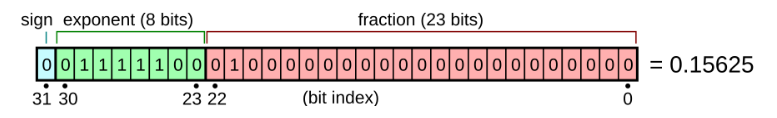
\includegraphics{float.png}
	\caption{an example of 32bit IEEE 754}
	\label{float}
\end{figure}


